\documentclass[doc,fignum,apacite,floatsintext]{apa6}
\usepackage[]{graphicx}
\usepackage{amsfonts}
\usepackage{amsmath}
\usepackage{geometry}
\usepackage{pifont}
\usepackage{adjustbox}
\usepackage{array}

\newcolumntype{R}[2]{%
    >{\adjustbox{angle=#1,lap=\width-(#2)}\bgroup}%
    l%
    <{\egroup}%
}
\newcommand*\rot{\multicolumn{1}{R{45}{1em}}}% no optional argument here, please!

\title{Referential precedents in spoken language comprehension: A review and meta-analysis}
\twoauthors{Edmundo Kronm\"{u}ller}{Dale J. Barr}
\twoaffiliations{Escuela de Psicolog\'{i}a, Pontificia Universidad Cat\'{o}lica de Chile}{Institute of Neuroscience and Psychology, University of Glasgow}

\abstract{Listeners' interpretations of referential expressions are influenced by established referring precedents---temporary conventions that associate linguistic expressions with discourse referents.  A number of psycholinguistic studies have sought to determine how much of precedent use reflects common ground (information that is believed to be shared) versus more egocentric, domain-general processes.  We provide a review and meta-analysis of visual-world eyetracking studies of precedent use, focusing on three principal effects: (1) a same speaker advantage for maintained precedents; (2) a different speaker advantage for broken precedents; and (3) an overall main effect of precedents.  Despite inconsistent claims in the literature, our combined analysis reveals surprisingly consistent evidence supporting the existence of all three effects, but with different temporal profiles.  These findings carry important implications for existing theoretical explanations of precedent phenomena, and challenge explanations of pragmatic phenomena solely based on common ground.\\[12pt] \centerline{\textbf{MANUSCRIPT UNDER REVIEW}, December 31, 2014}\\[12pt]}

\authornote{The authors thank Susan Brennan, Sarah Brown-Schmidt, and Sid Horton for sharing the original data from their studies for re-analysis.  In addition, we appreciate the helpful comments and criticism we received from Susan Brennan, Sid Horton, Editor Martin Pickering, and three anonymous reviewers.  This research was supported by Fondecyt-Chile grant (11100226) to the first author. Contact information: Edmundo Kronm\"{u}ller. Escuela de Psicolog\'{i}a, Pontificia Universidad Cat\'{o}lica de Chile. Avenida Vicu\~na Mackenna 4860, Macul, Santiago, Chile. Phone: +56 2 23545934. Fax: + 56 2 23545883. Email: ekr@uc.cl. Analysis scripts and data are available at \url{https://github.com/dalejbarr/precmeta}.}

\shorttitle{REFERENTIAL PRECEDENTS IN SPOKEN LANGUAGE}
\leftheader{E. Kronm\"{u}ller and D. J. Barr}
\keywords{PERSPECTIVE-TAKING, META-ANALYSIS, PRAGMATICS, CONVERSATION, EYE TRACKING}

\newcommand{\citetbl}[1]{\citeauthorNP{#1} \citeyear{#1}}

\begin{document}

\maketitle

\clearpage

One of the central questions in research on spoken language communication concerns how listeners derive context-specific interpretations from the linguistic form of spoken utterances.  Explaining how this derivation works is challenging because of there is a many-to-many mapping between linguistic utterances and a given speaker's communicative intention in a particular setting.  This complexity is evident in referential expressions such as \textit{the small candle}, which could be used by a speaker to refer to many different individual candles of varying size.  The linguistic content of such an utterance provides information only about the type of entity that is being referred to, leaving it up to the listener to decipher which particular token the speaker has in mind.  How do listeners identify relevant contextual information, and how is this information brought to bear on language processing?

Given that understanding a speaker's intended meaning is of paramount importance in dialogue, some theorists have argued for a central role of mutually shared information or \textit{common ground} \cite{clarkcarlson81,clarkmarshall81}.  Common ground is a special kind of shared information that is not only shared, but is also known (or believed) to be shared.  According to this view, listeners employ various \textit{co-presence heuristics} to identify common ground, which include \textit{perceptual co-presence}, \textit{linguistic co-presence}, and \textit{community membership}.  For example, listeners can know that a particular candle is the referent of \textit{small candle} because (1) it is the smallest candle that the interlocutors can see (perceptual co-presence); (2) it was previously mentioned in the current discourse in the presence of the current interlocutors (linguistic co-presence); or (3) the interlocutors are members of a community in which this particular candle is particularly salient (community membership).

An early, strong view of common ground assumed that resolution of spoken references is optimally efficient to the extent that listeners restricting the information they consider to their common ground with the speaker \cite{clarkcarlson81}.  However, studies have failed to support this strong view \cite{keysaretal00}, and some have presented evidence that the effect of common ground is probabilistic and partial rather than deterministic and absolute \cite{hannaetal03,nadigsedivy02}.  In other words, knowing that certain information is in common ground makes this information more likely to be used, without imposing an absolute restriction.  This view is influenced by the more general \textit{constraint-based view} of language comprehension, which regards interpretation as a constraint-satisfaction process, in which multiple cues are probabilistically weighted, with those interpretations that best satisfy the combination of cues winning out \cite{macdonaldetal94,tanenhaustrueswell95}.  Within this framework, common ground is but one of multiple cues integrated simultaneously during processing.  This view assumes that listeners actively track common ground, and that its effect on interpretation will be proportional to its contextual salience and reliability.  Furthermore, this view assumes no limit on listeners' ability to integrate this information with incoming speech at any stage of processing.  Thus, common ground should modulate language processing routinely, and should do so from the earliest moments of comprehension.

An alternative view assumes a more peripheral role for common ground in referential interpretation, viewing interpretation as based on various strategies and heuristics that are deployed largely egocentrically, i.e., without reference to the beliefs and intentions of the speaker \cite{keysaretal00,pickeringgarrod04}.  Successful interpretation may be the result of ordinary memory processes such as episodic priming and encoding specificity \cite{BarrJacksonPhillips2014,hortongerrig05a} or the deployment of heuristics that exploit regularities in language use, such as the association between discourse-novel expressions and discourse-novel referents \cite{kronmullerbarr07} or the use of a pronoun to refer to a salient entity \cite{FukumuraVanGompel2012}.  In short, reference resolution is assumed to involve an eclectic set of domain-general systems whose operations have been adapted to the demands of conversation.  This view does not rule out the possibility of common ground modulating interpretation, but assumes that it plays a more limited role, with some proponents arguing that situational assessments do not constrain certain low-level linguistic processes such as lexical access \cite{barr08b}.

One way researchers have sought to distinguish these views is by investigating the nature of discourse effects on reference resolution.  How do listeners make use of the conversational history of referring---the discourse record---to resolve references?  Forming a key part of the discourse record are the temporary referring conventions that interlocutors establish during a conversation, known as \textit{referential precedents} (or conceptual pacts; \citeNP{brennanclark96}).  When speakers introduce a referent into discourse, they choose from among a variety of conceptual perspectives on the referent that can be encoded using the conventions of language \cite{brown58}.  For example, the same object could be called a dime, a coin, money, a metal object, etc.  Because language is a cooperative activity, settling upon a particular way of describing a referent creates an expectation that the interlocutors will continue referring to that referent in the same way throughout the discourse.  Furthermore, participants in a dialogue will also come to expect that speakers will not use the same expression to refer to a different referent.  Referential communication studies show that speakers, by and large, fulfill these expectations \cite{brennanclark96,GannBarr2014,VanDerWege2009}.

Referential precedents not only reduce linguistic variability, making speech more predictable, but also provide a powerful basis for reducing ambiguity in reference resolution.  When speakers repeat a description they used earlier in the discourse, they are likely to be referring to the same thing they referred to on the last occasion they used that description.  Likewise, when speakers use a description they have not used before, it is likely they are referring to something that has not yet been mentioned.  Listeners indeed have these expectations about speaker consistency, and these expectations powerfully influence comprehension \cite{barrkeysar02,metzingbrennan03}.  But to what extent does this influence reflect the probabilistic use of common ground versus more egocentrically-based memory phenomena?

To address this key question, researchers have examined the \textit{speaker specificity} of referential precedent use---that is, the extent to which the effect of a precedent depends on whether or not the precedent was established by the current speaker or by a different speaker.  Studies typically involve listeners who interact with two different speakers, establishing different interactional histories with each speaker and thus different knowledge of established precedents.  Listeners are given reason to believe that neither speaker is aware of the other speaker's precedents.  To the extent that precedents are speaker specific, they should have a stronger influence with the speaker who established them; to the extent they are speaker independent, the influence should be independent of the identity of the speaker.

Studies have looked at two main cases of precedent use: maintained and broken precedents.  Speakers are said to maintain a precedent when they re-use an expression they have already established as a means for referring to a given referent; for example, continuing to refer to a particular car as \textit{the sportscar}.  To the extent listeners expect speakers to be consistent, they should benefit from this repetition.  To the extent that precedent use is speaker specific, this benefit should be greater when the speaker who repeats the expression is the one who established it precedent in the first place, a prediction we refer to as the \textit{same speaker advantage for maintained precedents}.  Speakers are said to break a precedent when they refer to something using an expression that differs from how they referred to it before; for example, referring to something you called a \textit{sportscar} as the \textit{Ferrari}.  Breaking an established precedent violates listeners' expectations, and thus should elicit confusion and delay identification of the intended referent.  To the extent  precedent use is speaker-specific, breaking a precedent should be most confusing when the person who breaks it is the same one who established it in the first place.  While it would be perfectly expected that different speakers might independently arrive at different ways of describing a referent, under most circumstances it is uncooperative for a speaker to change how they refer to something.  Thus, broken precedents should be understood more easily when the precedent is not in common ground with the current speaker, an effect we refer to as the \textit{different speaker advantage for broken precedents}.

Despite considerable work testing the prediction of speaker specificity for maintained and broken precedents, substantial disagreement remains, leaving the existence as well as the time course of such effects unclear.  Early claims of complete speaker independence \cite{barrkeysar02} have gone unsupported by later studies \cite{metzingbrennan03,brownschmidt09}, which do indeed find speaker specific effects, at least under some circumstances.  Researchers have sought to explain the apparent heterogeneous findings in the literature in terms of differences in experimental methodology and data analysis.  In this paper, we present results from a meta-analysis that challenges the assumption of heterogeneous findings, revealing instead a surprisingly uniform set of phenomena.  Our analysis, which combined results from 10 published experiments using visual-world eyetracking \cite{cooper74,tanenhausetal95}, detected three main patterns, namely: (1) that the same speaker repetition benefit for maintained precedents arises from the earliest moments of comprehension; (2) that the different speaker novelty benefit for broken precedents emerges late, well after the onset of the precedent main effect; and finally (3) that much of the influence of precedents on comprehension reflects speaker-independent (and thus, egocentric) processing.  Although these results do not definitively support any existing theoretical position on partner-adaptation in language comprehension, they offer important constraints on theorizing, and point the way toward more definitive future studies.  In the next section, a review of the literature on precedent use in comprehension sets the stage for our analysis.

\subsection{Referential precedents and expectations of consistency}

Our review focuses on studies of spoken language comprehension using the visual-world eyetracking paradigm with adult populations, as these studies provide the clearest, most detailed picture of moment-by-moment processing in the typically developing adult.  Studies of precedent use in child populations \cite{GrahamSedivyKhu2014,MatthewsLievenTomasello2012} have generally yielded similar results to those we consider below.  In addition, we excluded from our analysis studies using neuroimaging \cite{BogelsEtAl2014} or that examine long-term naming conventions established outside of the experimental laboratory, such as conventions for proper names \cite{BarrJacksonPhillips2014}.  Where relevant, we describe the results of these studies during our review of the main visual-world eyetracking studies on discourse conventions with adults.

The visual-world eyetracking paradigm \cite{cooper74,tanenhausetal95} is a methodology that is well-suited to investigating precedent use in spoken language comprehension.  This approach enables the measurement of listeners' moment-by-moment comprehension in conversational settings in a relatively unobtrusive manner.  In a typical visual-world eyetracking study, listeners' gazes are monitored while they participate in a collaborative task that requires them to follow a speaker's spoken instructions to manipulate objects, which can either be actual physical objects located in a display apparatus, or pictures of objects shown on a computer monitor.  On a typical trial, the speaker will mention a particular intended referent or \textit{target object}, such as \textit{the small candle}.  

There are various ways to measure and interpret visual behaviour during language processing.  Early studies using visual-world eyetracking usually measured the latency of eye gaze to target objects relative to the onset of a referential description \cite{altmannkamide99,keysaretal00,tanenhausetal95}.  For example, in Experiment~2 of \citeA{barrkeysar02}, listeners' latency to fixate the target was measured as a function of whether or not a precedent had been established, and whether or not the precedent was in common ground with the current speaker.  However, a more complete picture of processing can be obtained by calculating the moment-by-moment probability of gazing at the objects in the display \cite{allopennamagnusontanenhaus98}.  More recent studies on precedent use have tended to report and base statistical inferences on these more detailed gaze probability profiles.  Typically, the researcher computes a \textit{target advantage score} over a sequence of time windows, defined as the difference between the probability of gazing at the target object and the average probability of gazing at any other object within a given display.  This score is calculated for each condition over a series of time-bins (e.g., 50~ms) and typically presented in a graph, while statistical inferences are generally performed on larger-sized time-windows (e.g., 300~ms) in order to minimize the number of statistical tests.

Experiments on precedent use in comprehension require an experimental structure in which precedents are introduced (establishment phase) and then referred to again during later (in a test phase).  It is usually only the processing of the test phase utterances that is analyzed.  Studies on precedents usually use unconventional objects such as abstract tangram shapes or other kinds of unusual objects that lack conventional names in the language, as precedent effects are much more pronounced for these objects \cite{barrkeysar02}.  The wide variety of possible descriptions that can be given to these unusual objects encourages a reliance on referential precedents.  For example, a speaker could establish a precedent to refer to an object as ``the blueprint,'' but that same object could be called ``the spaceship'' or even be given a structural description such as, ``lots of white lines forming different shapes.''  The large number of ways that speakers could describe these objects makes it unlikely that two speakers would by chance arrive at precisely the same description.  The use of unconventional objects also avoids the potential problem of objects having preferred labels in everyday language.

The first visual-world study on precedent use in language comprehension \cite{barrkeysar02} presented findings from three experiments.  Experiment~1 found evidence that listeners benefitted greatly from established precedents, with referential search shortened by about 1300~ms when precedents were maintained.  Experiments~2 and~3 probed the extent to which this benefit was attributable to common ground by having listeners interpret expressions from two different speakers (male and female).  Experiment~2 sought evidence for the same speaker advantage for maintained precedents.  One of the speakers interacted live with the listener, working together to rearrange objects in a vertical set of shelves.  The other speaker gave instructions that were pre-recorded, and was only heard by the listener through a set of headphones.  On test trials, the live speaker referred to a target object under one of four conditions created by combining two factors: (1) whether or not a precedent had been established for the target; and (2) the identity of the speaker who established it, which was either the same as the current speaker (i.e., the live speaker) or a different speaker (i.e., the pre-recorded speaker).  To the extent precedent use is speaker specific, the effect of precedent should be larger when the precedent is in common ground.  An analysis of the latency of fixation on the target found a large benefit of precedents, with listeners identifying the target about 1500~ms faster when they could rely on a precedent.  However, there was no evidence that this advantage was any larger when the precedent was in common ground than when it was not (a difference of 50~ms that was not statistically reliable).  However, this conclusion is limited because it only considered the latency of the final fixation on the target, and thus might miss out on any effects that are early and transitory in nature.

Experiment~3 of \citeA{barrkeysar02} examined the role of precedents in listeners' expectations about the level of specificity that speakers would use when talking about conventional objects.  For example, one and the same car can be referred to as \textit{the vehicle} (superordinate level), \textit{the car} (basic level), or \textit{the sportscar} (subordinate level).  Despite the overwhelming tendency for speakers to refer to objects at the basic level, \citeA{brennanclark96} showed that if speakers entrained on subordinate level terms for referents that were paired with another member of the same basic-level category (e.g., referring to a car as \textit{the sportscar} to distinguish it from a station wagon) they would tend to persist in using these subordinate-level terms even in contexts where the basic level term would be sufficient (e.g., continuing to call it \textit{the sportscar} even though it was the only car).  Based on this finding, in Experiment~3, \citeA{barrkeysar02} asked whether listeners expect speakers to be overly specific, and whether such expectations were driven by common ground, or by their own egocentric experience.  

To test this, pairs of pictures from different categories were identified such that the basic-level name for one of the pictures (car) overlapped phonologically with the onset of the subordinate-level name for the other member of the pair (carnation), but where there was also no overlap between the subordinate level name of the former (sportscar) and the basic-level name of the latter (flower).  Listeners heard references from two different speakers, with half of the listeners led to believe that speakers spoke to them live over an internet link from another room (in reality, all speech was pre-recorded).\footnote{There was no evidence that listeners who believed they were hearing live speech performed any differently from listeners who believed they heard recordings, so this factor was ignored in the analysis.}  During the first part of the experiment, listeners heard a female speaker entrain on subordinate-level names for the objects (sportscar and carnation).  Each member of a picture pair appeared alongside another member of the same category (e.g., two cars or two flowers), requiring the speaker to entrain on subordinate level descriptions.  In the second part of the experiment, listeners either continued with the female speaker or with a male speaker who had just arrived, and who therefore would have no knowledge of the objects or of the precedents established by the original speaker.  Pairs of objects appeared together in the same display so that the basic level names would be sufficient to identify targets, and speakers referred to them using the basic level names, thus breaking the subordinate-level precedent.  For example, they viewed the car (entrained as \textit{sportscar}) and flower (entrained as \textit{carnation}) and heard the speaker say the word ``car''.  To the extent that they expect speakers to follow established precedents, they should show a tendency to gaze at the carnation upon hearing ``car''; to the extent these expectations are speaker specific, this tendency to gaze at the carnation should be stronger with the same speaker than with the new speaker.  Although listeners clearly expected speakers to continue using subordinate-level terms, there was no evidence that they expected this more strongly in the case of the same speaker.  

A subsequent study by \citeA{metzingbrennan03} examined the issue of broken precedents in more depth, focusing on unusual objects lacking conventional names in the language.  In their experiments, participants interacted with two live speakers (one male and one female) who swapped roles with one another, entering and exiting the room so that the listener would have no reason to believe they shared knowledge of precedents.  Speakers either maintained or broke established precedents, and the relevant precedents were either ones that they themselves had established or ones that a different speaker had established (forming the same speaker and different speaker conditions).  Metzing and Brennan analyzed latencies of first and final fixations to the target object.  As in Experiment~2 of \citeA{barrkeysar02}, they found no evidence for speaker-specific effects for maintained precedents.  However, they did find a different speaker advantage for broken precedents: namely, listeners were less delayed (\~286~ms) in identifying the target object when a speaker broke another speaker's precedent than when a speaker broke her (or his) own.  Indeed, there was no that listeners experienced any difficulty interpreting a new description of an old referent from a new partner.  When speakers broke their own precedents (versus one speaker breaking another's precedent), listeners looked more at non-target objects before looking at the target.

Inspired by this study, developmental researchers have also begun to investigate whether young children, like adults, expect consistency in adult referential behavior.  \citeA{MatthewsLievenTomasello2012} recorded video of children between three and five years old as they performed a referential communication task similar to \citeA{metzingbrennan03} with two different adult experimenters who instructed them to manipulate objects in a set of vertical shelves.  The experiment had a similar design to the study by Metzing and Brennan, with the same or a different experimenter either maintaining or breaking precedents established earlier in the experiment.  As a measure of interpretation, \citeA{MatthewsLievenTomasello2012} measured the time it took children to touch objects mentioned by the adult experimenter.  Children exhibited confusion when they heard new expressions for old referents, even when listening to the new speaker, but they showed most confusion when precedents were violated by the same speaker.  Interestingly, children often verbally protested against the speaker's use of the new term, even with the new partner.  It was clear that this behavior was the result of the precedent, as pre-experiment norming had shown that each term was equally good for describing the target.

A similar study by \citeA{GrahamSedivyKhu2014} used visual-world eyetracking with four-year-old children as they listened to two adult experimenters and viewed pairs of pictures on a computer screen.  In the establishment phase, one of the two experimenters established a particular way of referring to a given target object (e.g., the striped ball), and in the later test phase, that object was referred to once again using either the same adjective (striped) or a different adjective (yellow), and by either the same or a different speaker.  All referring expressions used a similar expression format: a head noun preceded by a modifying adjective.  Evidence for speaker-specificity emerged at the head noun, with a reliable difference between maintained versus broken precedents only in the case of the same speaker.  It is not possible to say whether there was a same speaker advantage for maintained precedents or a different speaker advantage for broken precedents, as these effects were not tested in the statistical analysis.  However, the graphs of the observed effects suggests some numerical support for the same speaker advantage.

A study by \citeA{kronmullerbarr07} that used visual world eyetracking with adult participants sought to follow up on the findings of \citeA{metzingbrennan03}.  Because \citeA{metzingbrennan03} reported only gaze latencies, \citeA{kronmullerbarr07} noted that the findings could not distinguish between two different effect profiles for the speaker-specific effect, each of which would carry distinct theoretical implications.  First, they noted that violating a precedent is confusing because of the phenomenon of preemption---the established association of a particular referent with a particular expression preempts the association of a new expression with that same referent within the discourse.  The different speaker advantage for broken precedents could arise from two possible sources: (1) speaker-specific preemption, in which listeners only experience preemption from precedents in common ground; or (2) speaker-independent preemption, followed by speaker-specific correction, a pattern they called \textit{recovery from preemption}.  The recovery-from-preemption explanation assumes that listeners experience preemption from any available precedent regardless of whether or not it is in common ground with the current speaker.  Under this account, the different speaker advantage emerges because listeners recover from this preemption more easily when the precedent is not in common ground, as this fact gives them reason to suspend their expectations of consistency.  Thus, when listeners hear a new expression for an old referent, there should be a period in which looks to the target are inhibited regardless of whether the precedent is in common ground, followed by a correction in which looks to the target rise faster in the different speaker case.

To distinguish these possibilities, \citeA{kronmullerbarr07} collected time-course data from two experiments in which listeners heard pre-recorded descriptions of unconventional referents from two speakers (one male and one female).  In Experiment~1, listeners searched for the target within an array that contained a varying number of objects, typically around eight.  Like in \citeA{metzingbrennan03}, listeners heard expressions that either maintained or violated established precedents, which in turn were either in or not in their common ground with the current speaker.  Consistent with recovery from preemption, listeners showed an early advantage for maintained precedents over broken precedents that was not modulated by speaker (emerging in 300--600~ms), with the different speaker advantage not emerging until much later, around 1500~ms.  A second experiment simplified referential search by using only three objects in each display, including the target, a previously mentioned non-target object, and an unmentioned object.  Furthermore, for half of the trials in Experiment~2, listeners had to maintain a string of digits in working memory, inducing a kind of cognitive load.  The hypothesis was that the load manipulation would have greater impact on the correction process than on the early partner-independent preemption effect.  Confirming these expectations, the advantage for maintained over broken precedents was apparent as early as 300~ms in both load conditions, with the different speaker advantage for broken precedents emerging only at around 900~ms, but only in the condition where listeners were not under load.  In the load condition, a post hoc analysis only found a recovery process extremely late in processing (after 2400~ms).

\citeA{brennanhanna09} later attributed the delay in the different speaker advantage that \citeA{kronmullerbarr07} observed to their use of a noninteractive paradigm, in which listeners heard pre-recorded expressions from non-present speakers.  From the point of view of collaborative models, interactivity is important since it is only possible to effectively ``ground'' a referential expression with a co-present interlocutor.  This would imply that common ground is established more weakly (if it can be said to be established at all) in a noninteractive setting.  As a result, Brennan and Hanna argue, effects of common ground might be smaller and possibly emerge later as compared to an interactive setting.  To test this idea, they revisited the data from \citeA{metzingbrennan03}, which was conducted in an interactive setting with live speakers, and performed a bin-by-bin analysis, similar to that used by \citeauthor{kronmullerbarr07}.  They found less interference for broken precedents with the new speaker at a relatively early time window, 600-900 ms.  However, consistent with recovery-from-preemption, this was preceded by a partner-independent main effect of precedent at 300-600 ms.  In other words, just as \citeA{kronmullerbarr07} found, the speaker-by-precedent interaction was preceded by a main effect of precedent.  Brennan and Hanna discounted this earlier main effect of precedent, noting that the target advantage score for this window was not yet statistically above zero.  Still, the presence of the main effect could be taken to indicate that the referential process had already begun.  It is therefore premature to view these results as undermining the evidence for recovery from preemption, especially in light of the fact that interactivity was far from the only difference between the experiments (see Table~\ref{t:bigtable}).

Findings from \citeA{shintelkeysar07} further challenge the assumption that grounding and mutual acceptance as in live interaction yield larger effects of common ground.  In two experiments, \citeauthor{shintelkeysar07} held constant listeners' knowledge about precedents while manipulating their beliefs about whether these precedents were mutually known.  Listeners observed speakers establishing precedents in one of two conditions: co-present with the speaker or not co-present (watching a video of the speaker over a video link).  It is only in the former case that the precedent can truly be said to be part of the common ground.  In the latter case, the listener knows what preferences the speaker has for referring to objects, but the precedents have not been mutually agreed upon.  An analysis of eye movement latencies found that listeners were delayed when speakers failed to be consistent in how they spoke about referents, but the magnitude of this delay did not appear to depend in any way on whether the precedent was mutual.  

The three experiments reported in \citeA{barr08b} were designed to address issues other than precedent use, but one of them, Experiment~3, included a setup in which a precedent was established for a target object (e.g., a bucket), either by a speaker referred to it again later, or by the experimenter.  The analysis focused on looks to a different object which was a phonological competitor to the target (e.g., a buckle), and which was also named either by the same or by a different speaker.  There was no evidence that the competitor interfered more when the precedent had been established by the same speaker than by the experimenter.  

Up to this point in the development of the literature, there seemed to be general agreement in the existence of a different speaker advantage for broken precedents, although it was not clear whether this effect was better explained by speaker-specific preemption or by recovery from preemption.  It was also the case that every attempt to find a same speaker advantage for maintained precedents had failed, suggesting that such an effect did not exist.  However, later studies eventually confirmed the same speaker advantage.  \citeA{barr08a} reanalyzed the maintained precedent conditions of Experiment~2 of \citeA{kronmullerbarr07} using multilevel logistic regression.  The analysis considered a time window from 300--450~ms, and found that the likelihood of gazing at the target increased at a faster rate when the speaker was the same than when the speaker was different.  Barr suggested that the original analysis by \citeA{kronmullerbarr07} failed to detect this difference due to the use of 300~ms time windows as well as due to the masking of the effect by an anticipatory effect in the opposite direction.  The analysis also found that the speaker specific advantage was not affected by a cognitive load manipulation, supporting the view that it was the result of episodic priming.  However, this effect was detected only while looking at a time-window defined post-hoc and without any statistical correction.

More convincing evidence for the same speaker advantage for maintained precedents was reported in a series of experiments by \citeA{brownschmidt09}.  Like \citeA{brennanhanna09}, Brown-Schmidt argued that it was the lack of interactivity in \citeA{kronmullerbarr07} that prevented the detection of the same speaker advantage for maintained precedents.  Participants in Brown-Schmidt's three experiments interacted with two different speakers, who were presented to participants as experimenters rather than as confederates.  The design was similar to \citeA{metzingbrennan03}, in that precedents were maintained or broken with the same or with a different speaker.  Experiment~1 supported the existence of a same speaker advantage for maintained precedents within the 200--600~ms window.  Although there was no different speaker advantage for broken precedents in any of the planned windows, an (uncorrected) post-hoc analysis on an unplanned time window from 180--300~ms did reveal some evidence for such an effect.  In a second version of this experiment, the live recordings from the experimental sessions were edited to remove all speech from the participant so that only the experimenter's speech remained.  This speech was then presented to a new set of participants who performed the task noninteractively.  No same speaker advantage for maintained precedents was obtained.  However, the same speaker advantage was once again demonstrated in a final experiment that once again involved live interaction with experimenters.  It is noteworthy that none of the experiments in this paper reported the different speaker advantage for broken precedents, apart from Experiment~1, in an uncorrected post-hoc analysis.

\citeA{HortonSlaten2012} provided further evidence for a same speaker advantage for maintained precedents across two experiments.  Listeners heard pre-recorded speakers describe referents during an early \textit{association} phase intended to build up knowledge of precedents and association them with particular speakers.  The experiments investigated whether speakers serve as retrieval cues for expression-referent associations stored in memory, as predicted by the ordinary memory account \cite{hortongerrig05a}.  The objects were tangram shapes designed to resemble various categories of objects (cats, people, cars, etc.).  During a later test phase, listeners viewed pairs of objects, both from the same category (e.g., two shapes that looked like cats).  Descriptions of these objects were of the form \textit{the cat with the very long tail}, such that the utterance would be ambiguous at the head noun (e.g. cat).  In the between-speaker condition, each picture had been previously associated with descriptions from different speaker.  In the within-speaker condition, both of the pictures forming a given pair had been associated with the same speaker, such that listeners would be unable to identify the referent until they heard linguistically disambiguating information.  The factor of between- versus within-speaker associations was crossed with the factor of speaker, which referred to whether the target was described by the same speaker who had originally established the association or by the other speaker.  Two experiments detected a same speaker advantage for maintained precedents: listeners in the between-speaker association condition looked at the target sooner when it was described by the same speaker.

To summarize, studies on precedent use in spoken language comprehension generally support the idea that listeners expect speakers to be consistent, and that when speakers conform to these expectations, comprehension is facilitated.  However, the mechanisms underlying these effects are not clearly understood.  To the extent that precedent effects are supported by common ground, there should be robust speaker effects: a same speaker advantage for maintained precedents and a different speaker advantage for broken precedents.  But these effects appear in some studies and not others.  It is possible that these speaker effects exist but are fairly small, thus accounting for the fact that they are not always detected.  Furthermore, the time course of these effects, when they appear, has yet to be definitively established.  One powerful way to address these problems is to combine effects across studies in a meta analysis.  In the next section, we provide further details about how we derived the effects used in the analysis, and also attempt to characterize the methodological dimensions on which the studies differ.

%%%%%%%%%%%%%%%%%%%%%%%%%%%%%%%%%%%%%%%%%%%%%%%%%%%%%%%%%%%%%%%%%%%%%%%%
%% The following section and the Method section need to be looked at
%% The big table describing all the experiments needs to be completed
%%%%%%%%%%%%%%%%%%%%%%%%%%%%%%%%%%%%%%%%%%%%%%%%%%%%%%%%%%%%%%%%%%%%%%%%

\section{Method}

The studies on precedents considered in the review above are shown in Table~\ref{t:bigtable}, which lists sample characteristics as well as methodological features of these studies.

\subsection{Composition of the sample of experiments}

Our meta-analysis focused on visual-world experiments with typically-developing adult participants, and thus we excluded experiments using young children as listeners \cite{GrahamSedivyKhu2014,MatthewsLievenTomasello2012}.  Although \citeA{BarrJacksonPhillips2014} used visual-world eyetracking with adults and addressed the issue of maintained referential precedents, we opted to exclude this experiment because the precedents under study were in the form of long-standing associations between proper names, voices, and persons, in contrast to the temporary discourse conventions used in standard experiments on precedent use.  Finally, we were unable to include \citeA{shintelkeysar07} because there was no manipulation of speaker (same or different), only a manipulation of maintained versus broken precedent, and whether the establishment of the precedent was in common ground with the speaker.

As reported in Table~\ref{t:bigtable}, our final sample included ten experiments.  Data from all ten experiments could address the same speaker advantage for maintained precedents, whereas only seven of the ten had appropriate manipulations to test for the different speaker advantage for broken precedents.  Finally, eight of the experiments provided appropriate baselines with which to test the main effect of precedent.

We contacted the authors of the original studies requesting access to the original raw data used in the analyses.  All authors we contacted complied with our request.  For the data from Metzing and Brennan (2003), we received the means used in the bin-by-bin analysis (300 ms time bins).  For all other experiments the data were divided into finer bin sizes (16, 24, 50, or 100~ms).  When calculating overall effects, we aligned all the time series using linear interpolation into 50 ms bins.  All of the data we obtained and our processing scripts are freely available for download at \url{http://github.com/dalejbarr/precmeta}.\footnote{For the Editor and Reviewers: We are waiting for written confirmation from the authors to allowing us to post their data for public access.}

We included both experiments from \citeA{kronmullerbarr07}, but separated out the data from the (within-subject) cognitive load conditions, treating them as though they were separate experiments, as load had a strong impact on processing.  Data for looks to the target from Experiment~3 of \citeA{barr08b} were also included, as these data can be used to test for the same speaker advantage for maintained precedents, even though this was not the main goal of the experiment.

Experiments~2 and~3 of \citeA{barrkeysar02} both contain speaker manipulations, but only Experiment~2 provides clear data for our analysis.  Experiment~3 could not contribute unambiguously to our analysis because the speech was temporarily ambiguous between maintaining and breaking the precedent; that is, it would be potentially unclear to listeners whether ``car'' was the first syllable of the subordinate-level term \textit{carnation} (maintaining the precedent) or just the basic-level term \textit{car}.  A further, more compelling motivation for excluding this study was that it involved breaking a precedent from a subordinate-level name to a basic-level conventional name for an object.  The use of conventional labels means that all ambiguity is resolved by the input (e.g., hearing 'car' when you expect 'sportscar'/'carnation' nonetheless leaves no doubt which of the two objects the speaker is referring to).  This is very different from the novel descriptions of novel objects used in experiments such as \citeA{brownschmidt09} and \citeA{metzingbrennan03}, where there was no existing conventional association between the label/expression and the referent.  In these latter cases, the ambiguity will be more difficult to resolve as it is based on a calculation of semantic similarity and not guided by conventional association.  This creates opportunities for the influence of common ground that are lacking in the case of precedents that are broken toward conventional names.

\subsection{Characteristics of the experiments}

In addition to variation in sample size, there are some important differences that are related to the many possible methodological and analytical variations on the basic paradigm.  Some of these differences are summarized in Table~\ref{t:bigtable}.  We define and review these differences here.

\subsubsection{Live Interaction}
Some experiments involved live interaction between speakers and listeners while in others, listeners heard pre-recorded speech. There are pros and cons to each of these alternatives. Live interaction is more naturalistic, representing what happens in a everyday face-to-face conversation. However, live interaction also adds variability to data since every critical expression is a unique token with different acoustic characteristics.  In contrast, pre-recorded expressions allow use of exactly the same expression for each test trial in all different conditions, reducing variability and thus increasing power.

\subsubsection{Confederate Identity Masked}
Independently of whether experiments use pre-recorded versus live speech, experiments varied in how the social identities of the speakers were presented to participants.  In some experiments, the fact that the speakers were associates of the lab was masked, with participants led to believe that the speakers were either previous participants in the experiment (in the case of pre-recorded speech) or that they were actual participants (in the case of live interaction).  This is generally done so that listeners will have the appropriate cooperative expectations about participants' speech.  The exceptions are \citeA{metzingbrennan03} and \citeA{brownschmidt09}, where speakers were presented as experimenters or lab assistants.  It is possible that making speakers' affiliation with the lab explicit could affect listeners' expectations of cooperativity.

\subsubsection{Speakers Blind to Condition}
Experiments differed in the knowledge of the speakers related to what condition a given test trial appears in (maintained versus broken, same versus different speaker). A criticism that is applicable to studies using live interaction is that speakers generally know whether they are using the same or a different expression to refer to an object (at least in the same-speaker condition), and this could potentially influence their linguistic performance.  Breaking one's own precedent is uncooperative and thus a face-threatening act.  It is possible that this knowledge could influence speakers' prosody or fluency in delivering the critical utterance, which creates a potential confound.

\subsubsection{Fixed Speaker at Test}
The test expressions used in experiments also vary in terms of how the speaker manipulation was implemented for a given experimental item.  For most experiments considered in the meta-analysis, the test utterance for a given item was produced by a single speaker in all conditions, with the identity of the speaker (same/different) implemented by varying the identity of the speaker who established the precedent.  Another method is to manipulate the identity of the speaker at test.  Experiments that follow this latter strategy will have additional variability in measurement due to variation in the acoustic realization of the same expression by different speakers.

\subsubsection{Fixed Expression at Test}
Another variation was how the maintained versus broken precedent manipulation was implemented.  In the broken precedent condition, the expression at test was a different expression from the one used previously.  The best way to accomplish this is to hold the test expression constant (since that is where the measurements take place) and vary the identity of the precedent established earlier.  So for example, if the test expression is \textit{the tent}, then the precedent would consistent of \textit{tent} in the maintained condition versus, for instance \textit{folded paper} in the broken condition.  The alternative would be to hold the established precedent constant as \textit{tent}, and break it by using \textit{folded paper} as the test expression.  Experiments following the latter approach will have additional variability in measurement due to variation in the linguistic form of the test expression. 

\subsubsection{Fixed Expression Format}
Another way to control variability and thus increase power is to use the same expression syntax across all items used in the experiment; by, for example, having all test expressions of the format \textit{determiner+adjective+noun}, e.g., \textit{the multicolored squiggle}.  Most experiments have different syntactic constructions for different items, which would add variability to the measurement of the time-course of the various effects.

\subsubsection{Time-Course Analysis}
Finally, experiments varied in the way data and results were presented in the paper and also in the statistical techniques used to analyze those data. Most experiments presented time course eye-tracking data in graphs as well as for the main analysis.  Two of the early publications presented data in terms of fixation latencies \cite{barrkeysar02,metzingbrennan03}, but access to the original data make it possible to include time-course data from these experiments in the meta-analysis.

\subsubsection{Baseline Control}
Listeners can sometimes develop expectations regarding the identity of the target object prior to hearing the test expression.  For example, listeners might expect speakers to refer to something they have not yet mentioned in the discourse, which would differ depending on the identity of the current speaker.  When listeners have such prior expectations, these introduce attentional biases to particular objects in a display (anticipatory baseline effects), which can be confounded with referential effects associated with the processing of the test expression \cite{barr08a,barrgannpierce11}.  Such effects can be controlled statistically by assessing the changes induced by the processing of the critical words in the expression relative to a earlier time-interval that serves as a baseline for attentional biases.  \citeA{barr08a} found evidence that the same-speaker advantage for maintained precedents was masked by an anticipatory baseline effect in the opposite direction.  To date, few studies have implemented such statistical controls.

\begin{table}[htp]
\caption{Experimental datasets, effects detected, and properties of the experimental setups}
\label{t:bigtable}
\begin{footnotesize}
\begin{tabular}{lc|rrr|rrr|rrrrrrrr}
\multicolumn{2}{c}{\hspace{2pt}}& 
\rot{No. subjects} &
\rot{No. items} &
\rot{No. cells in design} &
\rot{Main effect of precedent} & 
\rot{Same-speaker advantage, maintained} &
\rot{Different-speaker advantage, broken} &
\rot{Live Interaction} &
\rot{Confederate identity masked} &
\rot{Speakers blind to condition} &
\rot{Fixed speaker at test} &
\rot{Fixed expression at test} &
\rot{Fixed expression format} &
\rot{Time-course analysis} &
\rot{Baseline control} \\ \thickline
\multicolumn{1}{c}{Article} & Exp. & \multicolumn{3}{c|}{Sample} & \multicolumn{3}{c|}{Effects detected} & \multicolumn{8}{c}{Characteristics of the experiment} \\ \hline

\citetbl{barrkeysar02} & 2 & 36 & 12 & 4 & \ding{51} & \ding{55} & ---  & \ding{51} & \ding{51} & \ding{51} & \ding{51} & \ding{51} & \ding{55} & $^c$\ding{51} & \ding{55} \\


\citetbl{metzingbrennan03} & 1 & 24 & 8 & 4 & \ding{51} & \ding{55} & \ding{51} & \ding{51} & \ding{55} & \ding{55} & \ding{55} &  \ding{55} & \ding{55}  & $^c$\ding{51} & \ding{55} \\


\citetbl{kronmullerbarr07} 
& 1 & 52 & 8 & 4 & \ding{51} & \ding{55} & \ding{51} & \ding{55} & \ding{51} & \ding{51} & \ding{51} &  \ding{51} & \ding{51}& \ding{51}  & \ding{55} \\

\multicolumn{1}{r}{No Cognitive Load} 
& 2 & 56 & 16 & 4 & \ding{51} & $^a$\ding{51} & \ding{51}  & \ding{55} & \ding{51} & \ding{51} & \ding{51} &  \ding{51} & \ding{55} & \ding{51} & $^a$\ding{51} \\

\multicolumn{1}{r}{Cognitive Load} 
& 2 & 56 & 16 & 4 & \ding{51} & $^a$\ding{51} & $^b$\ding{51}  & \ding{55} & \ding{51} & \ding{51} & \ding{51} &  \ding{51} & \ding{55} & \ding{51}& $^a$\ding{51} \\


\citetbl{barr08b} & 3 & 36 & 24 & 6 & --- & \ding{55} & ---  & \ding{55} & \ding{51} & \ding{51} & \ding{51} & \ding{51} & \ding{55} & \ding{51} & \ding{51} \\


\citetbl{brownschmidt09} 
& 1a & 48& 16& 4 &  \ding{51} & \ding{51} & $^b$\ding{51} & \ding{51} & \ding{55} & \ding{55} & \ding{51} & \ding{51} & \ding{51} & \ding{51}  & \ding{55}\\
& 1b & 48& 16& 4 & \ding{51} & \ding{55} & \ding{55}  & \ding{55} & \ding{55} & \ding{55} & \ding{51} & \ding{51}& \ding{51}& \ding{51}&\ding{55} \\
& 2 & 32& 32& 4 & \ding{51} & \ding{51} & \ding{55}& \ding{51} & \ding{55} & \ding{55} & \ding{51} & \ding{51} & \ding{51}  & \ding{51} & \ding{55}\\


\citetbl{HortonSlaten2012} & 1 & 32 & 16 & 4 & --- & \ding{51} & ---  & \ding{55} & \ding{51} & \ding{51} & \ding{55} & \ding{55} & \ding{51} & \ding{51} & \ding{55} \\ \hline


\multicolumn{16}{c}{Additional experiments not included in the analysis} \\ \hline

\citetbl{barrkeysar02} & 3 & 64 & 8 & 4 & \ding{51} & $^h$\ding{55} & $^h$\ding{55}  & \ding{55} & \ding{51} & \ding{55} & \ding{55} & \ding{51} & \ding{51} & \ding{51} & \ding{55} \\

\citetbl{shintelkeysar07} 
& 1 & 36 & 10 & 4 & $^g$\ding{51} & --- & ---  & \ding{51} & \ding{51} & \ding{55} & \ding{51} & \ding{55} & \ding{55} & \ding{55}& \ding{55} \\
& 2 & 39 & 12 & 6 & $^g$\ding{51} & --- & ---  & \ding{51} & \ding{51} & \ding{55} & \ding{51} & \ding{55} & \ding{55} & \ding{55}& \ding{55} \\

\shortciteA{MatthewsLievenTomasello2012}
& 1 & $^d$126 & 8 & 4 & $^{g}$\ding{51} & \textit{nt} & \textit{nt}  & \ding{51} & \ding{55} & \ding{55} & \ding{55} & \ding{55} & \ding{55}& --- & --- \\

\shortciteA{BarrJacksonPhillips2014} & 1 & 20 & 48 & 8 & \ding{51} & \ding{51} & ---  & \ding{51} & $^{e}$\ding{51} & \ding{55} & \ding{55} & \ding{55} & \ding{51} & \ding{51}& \ding{51} \\

\shortciteA{GrahamSedivyKhu2014}  
& 1 & $^d$72 &  3 & 4 & \ding{51} & \textit{nt} & \textit{nt}  & \ding{51} & \ding{55} & \ding{55} & \ding{55} & \ding{55} & \ding{51} &\ding{51}& \ding{55} \\  \thickline


\end{tabular}\\
\ding{51} Yes; \ding{55} No; {---} Not Applicable; \textit{nt} Simple effects of speaker for each expression type not tested \\
$^a$ In post-hoc analysis with unplanned time windows and different statistical approach (see Barr, 2008a)\\
$^b$ In post-hoc analysis with unplanned time windows\\
$^c$ In later re-analysis, with original paper reporting fixation latencies\\
$^d$ Child sample \\
$^e$ Speaker was a na\"ive participant \\
$^g$ Response-time data \\
$^h$ Test expression temporarily ambiguous between maintaining/breaking precedent
\end{footnotesize}
\end{table}

\subsection{Definition and derivation of the three principal effects}

We now identify and discuss how we derived the three principal effects in the study. The first effect we calculated was the \textit{Main effect of precedent}. This effect reflects the facilitation (or inhibition) of processing due to maintaining (or breaking) an established precedent, independently of the identity of the speaker.  The interpretation of this main effect is ambiguous in the presence of an interaction, a complication that we discuss in the Results section.

The second effect of interest was the \textit{Same-speaker advantage for maintained precedents} which refers to the differential facilitation on comprehension that occurs when an expression is repeated by the same speaker compared to a different speaker. Finally, the third principal effect is the \textit{Different-speaker advantage for broken precedents}. This effect refers to the advantage that occurs when a new speaker refers to an old referent using a new expression, relative to an old speaker referring an old referent using a new expression (and thus violating his or her own precedent).

\begin{figure}
\caption{Design}
\label{fig:design}
\centerline{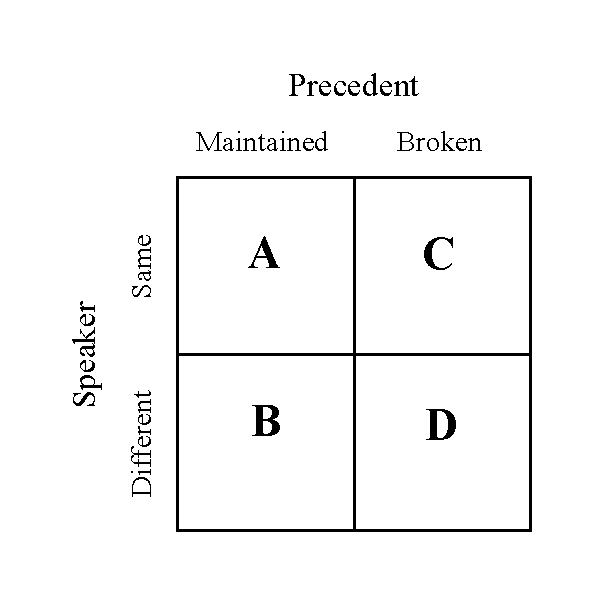
\includegraphics[scale=.6]{design.pdf}}
\end{figure}

In Figure \ref{fig:design} a schematic representation of the prototypical experimental design is depicted, combining the levels of the factor precedent (maintained vs. broken) and speaker (same vs. different).  To explain how the effects were derived, the cells of the design have been labeled A--D.  The Main effect of precedent is computed as the difference in the marginal means for the precedent manipulation, that is, $(A+B)/2-(C+D)/2$. The other two effects correspond to the two simple effects of the variable speaker in the two levels of the variable precedent. The same speaker advantage for maintained precedents corresponds to the simple effect of speaker when the precedent is maintained and is computed by substracting the different speaker maintained condition to the same speaker maintained condition $(A-B)$. The different speaker advantage for broken precedents is computed by substracting the same speaker broken precedent to the different speaker broken precedent $(D-C)$. 

\subsection{Estimation of effects and effect variability}

Meta-analyses often use dimensionless measures of effect size (such as Cohen's \(d\)) to combine information across disparate studies.  Dimensionless effect sizes are most useful when combining information from multiple studies for which only summary statistics are available, or that use different measures that are otherwise incommensurable.  The disadvantage of these statistics is that they are in themselves difficult to interpret except in a relative sense.

Given that all studies used the same measure (target advantage score) and given that we had access to all the original data, it seemed preferable to report effects in their original metric rather than as dimensionless statistics.  It could be argued that standardized measures might be preferable because they control for differences in sample size, but this is also not entirely true, inasmuch as the variability of effect size estimates themselves strongly depends on sample size.  Furthermore, most effect size measures depend on parametric assumptions about variability for their validity, where as nonparametric techniques for estimating effect variability rely on fewer assumptions.  Given these considerations, and the fact that relative rather than absolute effect sizes were of main interest, we used the full data to obtain the most precise parameter estimates possible instead of calculating standardized effect size measures.

We estimated variability in the parameter estimates for each time series by deriving 95\% confidence intervals from 10,000 bootstrap samples of the dataset.  We created resampled versions of the dataset by independently sampling subjects (with replacement) from each of the relevant studies, and then recalculating the effect under consideration.  Most of the data we had access to contained data aggregated up to the subject level, and thus we were unable to consider items as a random source of variation.

\citeA{barr08a} pointed out that anticipatory baseline effects---effects present prior to the onset of referential processing---create biases that can mask existing effects or create spurious effects.  To correct for these effects, we calculated the mean target advantage score for all bins in a series less than 200~ms after speech onset, and subtracting this value from the time series.  This was done only in the calculation of the overall (mean) trendline for each of the three effects, but not for the individual series associated with each study.

Data processing and visualization were performed using R \cite{R3.1}, with extensive use of add-on packages \texttt{dplyr} \cite{dplyr-0.3.0.9}, \texttt{tidyr} \cite{tidyr-0.2.0}, and \texttt{magrittr} \cite{magrittr-1.5} for reshaping and organizing the data, and \texttt{ggplot2} \cite{ggplot2} for creating graphs.

\section{Results and Discussion}

\begin{figure}
\caption{Temporal profiles of effects in individual experiments (colored lines) with overall baseline-corrected trendline (dark line) and confidence intervals based on 10,000 bootstrap samples.}
\label{fig:allfx}
\centerline{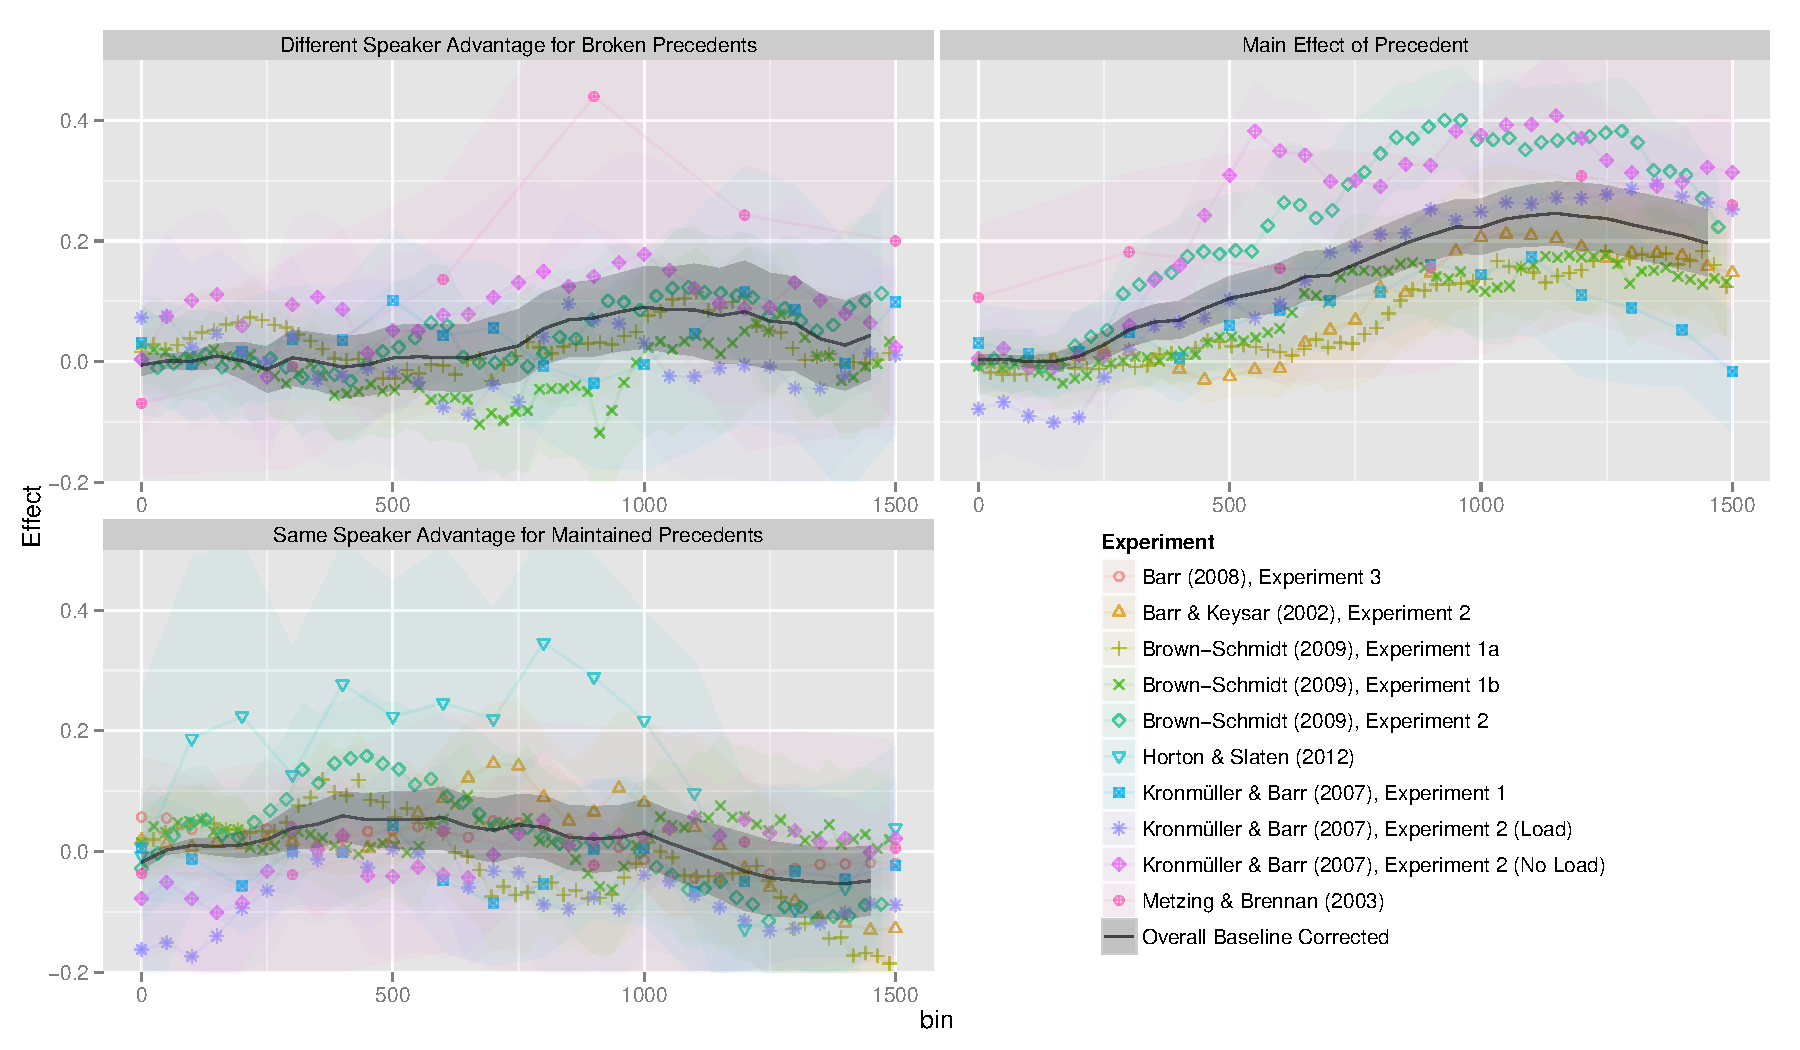
\includegraphics[width=6in]{alleffects.pdf}}
\end{figure}

Figure~\ref{fig:allfx} presents the effect profiles from the individual experiments, along with mean trendlines and 95\% confidence intervals derived from bootstrap resampling of the individual studies.  To enable comparison of the magnitudes of the three principal effects, Figure~\ref{fig:effsize} presents the main trendlines and confidence intervals together in a single graph.  The main effect of precedent emerged from the earliest moments, with an increasing trend starting at 200~ms that became reliable by 400~ms and remained so until the end of the analysis window.  The speaker effect for maintained precedents showed a similar early pattern, closely tracking the main effect of precedent until around 450~ms.  This pattern was consistent across experiments, with eight of ten showing a positively-sloped curve from 200~ms to 450~ms, the two exceptions being Experiment~1 of \citeA{kronmullerbarr07} and Experiment~1b of \citeA{brownschmidt09}.  Interestingly, from its peak at 450~ms, the effect gradually decayed, becoming statistically unreliable by 700~ms.  Curiously, it even seemed to show a reversal around 1200~ms, with listeners becoming slightly more likely to look at the target when a new speaker followed another speaker's precedent, but this was not statistically robust.  This analysis lends confidence to the existence of a same speaker advantage for maintained precedents, with the effect arising immediately but yielding only a transitory advantage.

\begin{figure}
\caption{Relative effect sizes of main effects and speaker effects.}
\label{fig:effsize}
\centerline{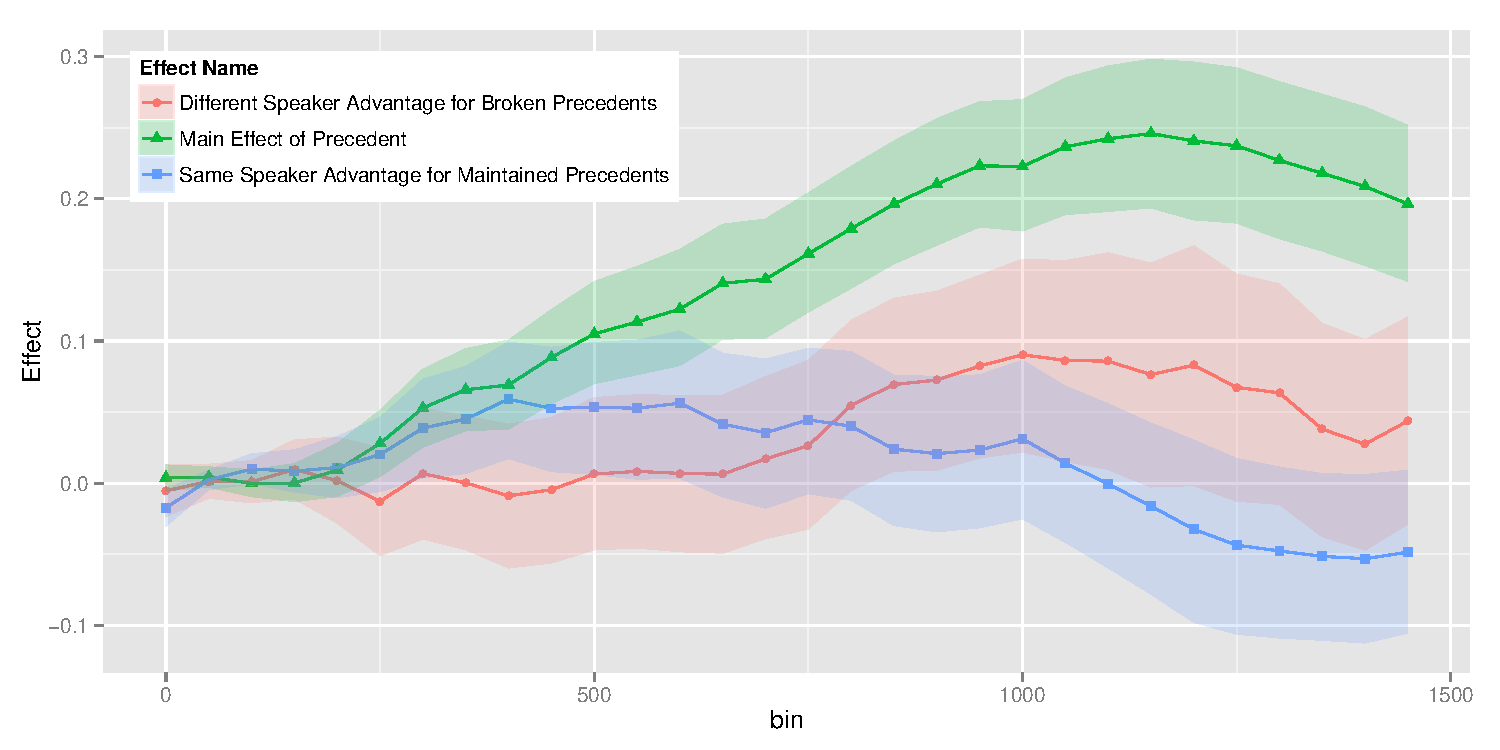
\includegraphics[width=6in]{releff.pdf}}
\end{figure}

The different speaker advantage for broken precedents, in contrast, had a drastically different overall temporal profile from either the main effect or the same speaker advantage for maintained precedents.  This effect emerged much later than the same-speaker advantage for maintained precedents, no earlier than 700~ms after speech onset, well past the peak of the same-speaker repetition benefit, and well after the onset of the precedent main effect.  The effect became reliable by 800~ms and showed a sustained effect that seemed to dip down slightly from 1250~ms.

The pattern was fairly consistent across the seven studies that we considered.  By about 1150~ms, all studies showed the same numerical benefit for different speakers excepting the Load condition of Kronm\"{u}ller and Barr (2007), Experiment 2.  Note that the non-interactive Experiment 1b of \citeA{brownschmidt09} also showed a weak effect.  The weak speaker effect in the former study can be explained by cognitive load impeding listeners' ability to use common ground.  The latter study had no load manipulation, but is unusual in how the speech stimuli were generated.  Unlike other studies, Brown-Schmidt's Experiment 1b used recorded speech from actual spontaneous dialogs between experimenters and actual participants, with the speech of the participants edited out.  Research indicates that hearing only half of a conversation imposes attentional demands on listeners \cite{EmbersonEtAl2010}.  Perhaps the use of such ``half-a-logues'' in Experiment 1b of \citeA{brownschmidt09} imposed attentional demands on listeners that, like the cognitive load manipulation in Experiment 2 of \citeA{kronmullerbarr07}, reduced the different speaker benefit for broken precedents.

\begin{figure}
\caption{Partner-specificity index mean experiment trendline and 95\% bootstrap confidence interval (shaded region).  Higher values reflect with greater partner-specificity.}
\label{fig:sspec}
\centerline{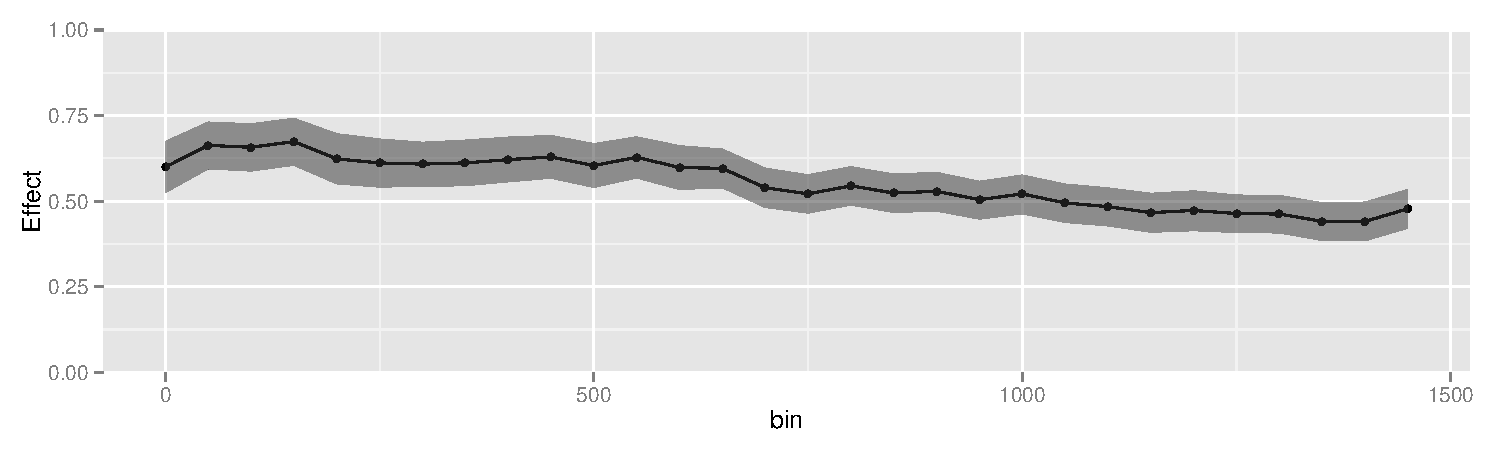
\includegraphics[width=6in]{psi.pdf}}
\end{figure}

Lastly, we note that across all studies, the effect that was largest and most consistently detected was the main effect of precedent---whether a precedent was maintained or broken \textit{for the listener}. Indeed, every single one of the experiments included in the analysis (Table~\ref{t:bigtable}) for which a precedent effect could be calculated reported a statistically significant main effect of precedent, in contrast to only 5/10 reporting a significant speaker effect for maintained precedents (one post-hoc, uncorrected), and 5/7 reporting the speaker effect for broken precedents (two post-hoc, uncorrected).

The interpretation of this main effect is complicated by the presence of the interaction between speaker and precedent (as embodied in the two speaker-specific effects).  What proportion of this main effect is driven by the interaction, and what proportion is independent?  To answer this question, we devised a ``partner-specificity index'' as follows.

One way to think of the main effect of precedent is as the mean of the two simple effects of precedent (maintained minus broken), one for each level of speaker conditions (same and different).  Denoting these two simple effects as $X_{same}$ and $X_{diff}$, the main effect $M$ is given by $M = \frac{X_{same}+X_{diff}}{2}$.  To the extent that precedent use is partner specific, $X_{same}$ will be greater than zero, and $X_{diff}$ will approach zero.  Complete partner specificity entails that $M=\frac{X_{same}}{2}$.  In contrast, complete partner independence implies that $X_{same}=X_{diff}$, and thus that $M=X_{same}$.  These observations suggest the possibility of creating an index of partner specificity using the following formula:

% \textbf{TODO: give formula}
$$\frac{2X_{same}}{X_{same} + X_{diff}}-1$$

\noindent where zero implies pure partner independence (both simple effects are equal) and one implies pure partner specificity.  The formula assumes that $X_{same} \ge 0$ and $X_{diff} \ge 0$, so in any case where either effect was negative, we set it to zero.  Also, the formula assumes that $X_{diff} \le X_{same}$, so in those cases where $X_{diff}$ exceeded $X_{same}$, we truncated it to equal $X_{same}$.

Figure~\ref{fig:sspec} shows the overall partner-specificity index plotted as a function of time, along with mean trendline and 95\% confidence interval.  The index ranged from 44\% to 67\%, with a mean of 55\% (median 54\%).  Thus, between 33\% and 56\% of the main effect of precedent is not explained by partner specificity, and can therefore only be attributable to partner-independent factors.

\section{General Discussion}

Our combined analysis of ten experiments on precedent use in comprehension detected a level of consistency that is surprising against the background of the contradictory findings and claims in the literature.  We found strong evidence to support the existence of three principal effects with distinct temporal profiles: an early but small and fleeting same-speaker advantage for maintained precedents, a later, sustained different-speaker advantage for broken precedents, and a strong and monotonically increasing main effect of precedent.

Against \citeA{barrkeysar02} and \citeA{metzingbrennan03}, and supporting \citeA{brownschmidt09}, there was clear evidence for a same-speaker advantage for maintained precedents, which was present from the earliest moments of comprehension, i.e. as soon as any referential commitment can be identified. Eight of the ten studies we considered exhibited a positive slope in the 200--450~ms window.  Without assuming the existence of the effect, it would be difficult to explain this consistency in timing and direction of the effect profile.  Our investigation also supports the existence of a different-speaker advantage for broken precedents, which in comparison to the speaker effect for maintained precedents, only emerged after a substantial delay.  The different-speaker advantage also appears statistically reliable in the combined analysis, despite not being reliably found in all individual studies testing for such an effect, such as in two of the three experiments in \citeA{brownschmidt09}.

In this section, we first consider some of the limitations of our study.  We then turn to what the differences in temporal patterning for the three effects might imply in terms of underlying mechanisms.  Next, we discuss possible methodological reasons why individual experiments may succeed or fail in detecting these effects, which appear robust in the aggregate.  Finally, we close with some practical implications of this study for how visual-world eyetracking data can best advance psychological theory about language comprehension in dialogue.

\subsection{Limitations}

One of the perennial problems with meta-analysis is publication bias and the well-known ``file drawer'' problem \cite{rosenthal1979file,sterling1959publication}, such that the set of published studies is not representative of the existence of effects and their magnitude.  
It can be difficult to correct for publication bias to get a true picture of the effect (but see \citeNP{SimonsohnSimmonsNelson2014}).  What might publication bias look like in research on precedent use in comprehension?  Typically, publication bias is usually though of in terms of the underrepresentation of null results in the literature.  It seems extremely unlikely that the main effect of precedent could result from publication bias, but what about the two speaker effects?  Effects that are the result of publication bias should have no consistent time course across studies.  In this regard, it seems unlikely that two effects with consistent and consistently distinct timecourses could result from publication bias.

Another potential concern with the analyses is the potential misestimation of the magnitude and time course of effects due to differences in stimuli and experimental setups across studies.  Some of the studies used brief, single word expressions while others used longer multiword expressions.  Furthermore, the studies varied in terms of the number of potential referents presented to the listener, and whether these were actual objects or computerized depictions of objects.  This means that the same effect is likely to have systematically different time courses across experiments.  If these differences are left unaccounted for when the time series are averaged together, then effects will be underestimated inasmuch as they get ``smeared'' across the time window.  This is just a more general version of the smearing that is likely to take place within a single experiment due to individual differences among subjects or among experimental items.  But we see no a priori reason to believe that the smearing would be more or less of a problem for any one of our effects than for any other, since they are all drawn from the same set of experiments, nearly all of which used the same test stimuli in all experimental conditions (see Table~\ref{t:bigtable}).  Thus, the smearing would make it more difficult to detect effects, but without any good arguments for why the smearing might impact one effect more than another, there is little reason to fear that it would compromise relative comparisons of their sizes or temporal patterning.

\subsection{Potential mechanisms underlying the effects}

Taking the effects at face value, what might their different temporal profiles imply for theories of language comprehension in dialogue?  Can these patterns be accounted for by constraint-based approaches, which assume that information is integrated in a fully interactive system as soon as it becomes available?  Or do they implicate multiple functionally distinct subsystems, with more limited interactions among the subsystems, and perhaps a more peripheral role of common ground?  Although our findings cannot provide definitive answers to these questions, they can constrain theorizing about potential underlying mechanisms and point the way toward future research.

We begin our discussion of these mechanisms by considering the same-speaker advantage for maintained precedents.  One view of this effect is that it reflects the immediate activation and integration of common ground with the semantics of the referring expression \cite{brownschmidt09}.  Immediate use of common ground has often been a prediction that has been used to distinguish constraint-based models from egocentric-first processing \cite{hannaetal03,nadigsedivy02}.  But if the effect reflects use of common ground, it is unclear why it would decay over time; unlike the other effects, which seem to mostly increase over the window, the same speaker advantage for maintained precedents completely dissipates by 1000~ms.  Under constraint-based models, which assume an evidence accumulation process, the probability of gazing at a given referential alternative at a given moment should reflect the totality of evidence accumulated for that alternative up to that moment.  In the context of the referential communication experiments reviewed above, evidence accumulation for the target is monotonic---the listener receives increasing evidence over time for the target.  So why is the peak effect of the social and linguistic information not sustained over the full interval, as seems to be the case for the two other principal effects?  It is as if the speaker information affects eye gaze behavior without contributing to the evidence accumulation process per se.

An alternative proposal that fits with the transitory nature of the effect assumes that the effect reflects episodic priming.  By episodic priming, we mean the phenomenon by which a cluster of associations stored in episodic memory associated with a stimulus are activated in a manner independent of conscious awareness \cite{TulvingSchacter1990}.  For instance, hearing a word repeated by the same speaker versus a different speaker can influence recognition memory for a word, implicating that listeners maintain detailed traces of the perceptual event associated with hearing a spoken word \cite{churchschacter94,goldinger96,mullennixpisonimartin89}.  In the case of referential language, it seems likely that such episodic traces will additionally contain information about the referent of the expression, such that hearing an expression will more strongly activate the referent associated with the expression on previous trials when it is spoken in the same voice.

Episodic priming better explains the transitory nature of the phenomenon than common ground.  Priming can lie outside of awareness and might be the result of a memory system that is functionally independent of the systems involved in linguistic interpretation.  The explanation in terms of episodic priming is also supported by the observation that the same-speaker advantage seems impervious to cognitive load.  A number of studies that suggest that accessing and using common ground requires effortful attention \cite{brown-schmidt09exec,nilsengraham09,rossnagel00}.  Experiment 2 of \citeA{kronmullerbarr07} tested the effects of load on the use of precedents, with half of the participants performed the task under cognitive load.  \citeA{barr08a}'s reanalysis of this experiment found an increasing slope from 300--450 ms for the same speaker condition, with no evidence that the effect was modulated by cognitive load.  In contrast, the load manipulation strongly influenced the different-speaker advantage for broken precedents.

This view of the same speaker advantage for maintained precedents is fully consistent with the \textit{ordinary memory} view of speaker specific processing in language use, according to which other language users can serve as memory cues to situationally-relevant information through a ``resonance'' memory process \cite{hortongerrig05a}.  To the extent that there is an overlap between information associated with a speaker and common ground, this process can serve as a cognitively efficient proxy for common ground.  Furthermore, it can serve as a starting point for more direct inferencing about common ground.  However, it is important not to directly identify speaker-specific associative memory with common ground, as the former depends merely on associations while the latter critically relies on mutual belief \cite{clarkmarshall81}.  When listeners witness a speaker choosing to refer to a piece of folded paper as ``the tent'', they will store an episode in memory that links together the speaker, the expression (in that speaker's voice), and the referent.  However, it is only in the case in which the listener knows that speaker knows that the listener has observed the labeling event, that the episode becomes part of the common ground; if there is no co-presence---e.g., if listeners secretly observed the labeling episode over a video link---then they have no basis for believing that the speaker knows that they know.  Speaker effects in precedent use may be independent of whether these higher-level links in the inference chain have been completed, and as such, may reflect basic memory operations or egocentric heuristics rather than common ground \cite{shintelkeysar07}.  

Another argument against conflating common ground with ordinary memory is that memory associations and common ground can point in different directions during language use, for instance in cases of direct quotation or simultaneous translation.  In such cases, what is relevant for interpretation is the common ground with the designer of the message rather than the information that happens to be associated with the person who is delivering the message.  In a study on proper names, \cite{BarrJacksonPhillips2014} found that people identified a target person based on a name (e.g., ``Kevin'') when the name was spoken by a friend with whom the target person was in common ground than by a stranger.  However, there was no evidence this facilitation was any smaller when the friend who spoken the name was not the source of the message---specifically, when the friend was directly quoting another speaker with whom the target person was \textit{not} in common ground.  Thus, the association between the friend's voice saying the name and the target person drove the facilitation, rather than the common ground.  It is also interesting to note that the time course of this facilitation was similar to that observed in the current study, and also exhibited a pattern of decay.

The different speaker advantage for broken precedents shows a strong contrast in temporal patterning to the same speaker advantage for maintained precedents, appearing much later and with less of a tendency toward decay.  The fact that the effect emerges long after the onset of the precedent main effect is consistent with the recovery-from-preemption proposal \cite{kronmullerbarr07}, in which listeners use common ground to recover from a partner-independent preemption effect.  Supporting the idea that this effect involves common ground, imposing cognitive load on listeners strongly attenuates this effect \cite{kronmullerbarr07}, consistent with many other studies (cited above) suggest that reasoning about common ground is effortful.  Pragmatic inferencing also seems implicated by the fact that the effect appears strongest on the first trial involving a broken precedent \cite{brennanhanna09,MatthewsLievenTomasello2012} and dissipates strongly on the next and subsequent trials.  This is consistent with listeners suspending their assumption that the speaker is cooperative.  In contrast, no such dissipation over trials has been reported for the speaker effect for maintained precedents.  Finally, studies suggest that, unlike for maintained precedents, the speaker knowledge being accessed to resolve broken precedents does contribute to the overall evidence accumulation process: specifically, whether or not the precedent is in common ground affects the rate of target selection, with listeners more likely to select the target in the different speaker condition \cite{kronmullerbarr07} (this comes with the caveat that the identity of the target is usually less ambiguous in the case where a precedent is maintained than when it is broken).

Further support for the recovery-from-preemption proposal comes from a recent neuroimaging study in which listeners' brain activity was observed using magnetoencephalography (MEG) while they heard speakers break precedents \cite{BogelsEtAl2014}.  Areas of the brain associated with mentalizing (e.g., ventromedial prefrontal cortex, right temporoparietal junction) seemed to be activated ``on demand'' to restore coherence after a pragmatic violation, instead of being activated in advance to calibrate listeners' expectations to their common ground with the current speaker.

The fact that this different speaker advantage occurs much later than the main effect would seem at first blush to pose difficulties for constraint-based accounts.  However, there are at least two ways in which constraint-based accounts could explain it.  One way is by assuming that is integrated immediately once it becomes available, but that its availability is itself slow.  This type of delayed-availability explanation has been pursued to reconcile apparent delays in the timing of top-down lexical effects relative to bottom-up acoustic effects in spoken word recognition \cite{magnusonetal03}.  Making such an explanation work in the current case requires assuming that the earlier same speaker advantage reflects episodic priming rather than common ground; otherwise, it would be implausible that common ground would be available earlier in one case than in another.  A better explanation would seem to be that the referential process itself is delayed in the broken precedent case.  This view is possible because for nearly all of the studies involving broken precedents, the main effect involves a comparison between maintained and broken precedents.  It is customarily assumed that the main effect, once it appears, reflects both facilitation in the maintained condition and inhibition in the broken condition.  But this need not be the case: the early part of the main effect could be driven solely by facilitation.  Thus, the onset of the different speaker advantage could, in fact, be concurrent with the onset of the earliest referential effects for broken precedents.  What would be necessary to resolve this ambiguity is a design including a neutral ``no precedent'' baseline against which the onset of referential processing could be assessed.  If there is no evidence for an interval prior to the onset of the different speaker advantage in which looks to the target are inhibited (in a partner-independent manner), this would support the constraint-based account.

Researchers studying precedent use in comprehension have almost single-mindedly focused their efforts on documenting the existence and timing of the above two speaker-specific effects, and in developing explanations for the observed patterns.  This is unfortunate since (as Figure~\ref{fig:effsize} indicates) speaker-specific factors explain at most half of the total effect of precedents on comprehension.  Thus in large part, listeners expect to hear descriptions conforming to established precedents due to factors that are unrelated to common ground or speaker-specificity, but the field is currently lacking a good explanation for what might give rise to this pragmatic effect.  It is possible that the speaker-independent share of the maintained precedent effect reflects priming due to the established symbolic association.  Alternatively, it may be the case that listeners are following a simple heuristic according to which old expressions are mapped to old referents and new expressions to new referent\cite{kronmullerbarr07}, without relying on any other information than discourse status, either new or old.  Simple heuristics for pragmatic inference would also be consistent with some approaches in the developmental literature that postulate that children have general biases guiding referential interpretation, such as the Mutual Exclusivity Bias, by which children assume that an object can not have two different labels \cite{markmanwachtel88}, or the Novel-Name Nameless-Category Principle \cite{mervisbertrand94} (c.f. \cite{diesendruck05,diesendruckmarkson01}).

An interesting possibility that has not been sufficiently explored is that speaker-independent precedent effects reflect listeners' use of a model of the behavior of a \textit{generic speaker}.  This idea is the comprehension counterpart to the \textit{generic listener} developed for production by \citeA{browndell87}.  Brown and Dell proposed that speakers might design their utterances to meet the informational needs of a generic listener---someone exactly like themselves who is lacking only the knowledge encoded by the utterance being planned---rather than the actual particular listener they are speaking to.  Similarly, it may be that listeners interpret utterances as if they were formulated by a generic speaker---someone sharing their knowledge exactly except for the to-be-decoded intended meaning of the message---rather than the actual particular speaker they are listening to.  In other words, listeners are engaging in the bare minimum of speaker modeling necessary to get pragmatic effects off the ground.  This account seems more appealing than simply invoking ``egocentrism'' to explain departures from fully cooperative listener behavior.  Such a negative definition of egocentrism is too underspecified to explain why there should be partner-independent pragmatic effects at all.  Egocentrism could mean anything from the listener not caring at all about the previous discourse history (and thus showing no effects of precedents) to using heuristic approximations to common ground to guide comprehension.  The fact that there are robust effects of precedents that are not attributable to common ground seems difficult to explain without listeners at least bringing to bear some kind of quasi-rational speaker model on the comprehension process.  We think this avenue is worth exploring in future research.

Because the debate in research on dialogue has centered around the question of whether partner-specific effects exist, any the field has not yet grappled with the towering effects related to speaker-independent pragmatic processing.  This is unfortunate because the partner-independent portion of the overall precedent effect is at least as large as that attributable to partner specific factors.  Theories of precedent use based on common ground alone have weak explanatory power, especially if, as we have argued, the early same-speaker advantage for maintained precedents reflects episodic priming rather than common ground.

In sum, while our findings can be explained by existing theoretical accounts, they point the way toward for further research than can better distinguish the accounts.  In particular, further studies are necessary to determine whether the early speaker advantage for maintained precedents reflects episodic priming or common ground.  Currently, the data better supports episodic priming, to the extent that such effects are not affected by load \cite{kronmullerbarr07}, are transitory in nature, and seem tied to perceptual characteristics of the message rather than common ground with the message designer \cite{BarrJacksonPhillips2014}.  Still, further experimentation is needed to better shore up this explanation.  The late different speaker advantage for broken precedents needs to be tested within a design containing a neutral baseline to distinguish recovery-from-preemption from merely delayed reference resolution.  Finally, new studies and theoretical development are needed to explain the partner-independent aspect of precedent effects.

%We believe that the distinct temporal profiles of the effects studied, taken together with findings from other studies, support the view that precedent effects are realized by a variety of underlying and functionally distinct cognitive mechanisms. In what follows, we suggest a central role for egocentric computations arising out of domain-general processes, compared to a less central role for common ground, mainly in monitoring and correction.  Specifically, we propose that the same-speaker advantage for maintained precedents, the different-speaker advantage for broken precedents, and the partner-independent main effect of precedents, respectively are the result of: (1) episodic priming; (2) a correction process involving invocation of common ground; and (3) predictions based on egocentric heuristics. We start by considering these explanations in turn and then we briefly discuss how this pattern of results can be explained by a constraint-based approach, as an alternative to our view that they are realized by different cognitive mechanisms.

%At some level, it may seem that our proposal of multiple cognitive mechanisms is compatible with a constraint-based approach. Indeed, these type of models don't deny that there are different processes providing different type of information\cite{brennanhanna09}, such as the acoustic and lexical effects in spoken word recognition in TRACE. The main proposal is that all the information is combine in a single-stage in a way that each individual processes can not have an output that is not influenced by the output of another process; and, as we said before, the character of this influence is probabilistic which is determined by the reliability, salience and availability of the informations constraints. Single stage Constraint-based models are reaction against modularity claims, where the output of some processes can not be influenced by other processes. We think, however, that some level of modularity might fit well with the pattern of results presented. As we argued, the partner-independent effect of precedent appears robust and impermeable to speaker-specific information. Such impermeability has been also found for lexical activation not being influenced by common ground, even when this last information is available and exerting effects on comprehension in the form of anticipation \cite{barr08b}.

%--It is hard to understand why the burden of proof is on the hands of the proposers of a multiple systems and even modular. One of the weekness of Constraint-based approaches is that they can easily accomodate post-hoc many different patterns of results. Contraint based-models, ironically, are hard to constrain by data. 

\subsection{Explaining inconsistency of the studies}

To orient future research on this topic, it is informative to consider some of the possible reasons why some studies have succeeded while others have failed to detect partner specific effects.  To begin, various factors may have conspired against the detection of the speaker-specific repetition benefit.  First, the effect is short lived, making it difficult to detect using fixation latency measures, such as those used in \citeA{barrkeysar02} and \citeA{metzingbrennan03}.  Second, in some cases, the effect is sometimes masked by anticipatory baseline effects in the opposite direction \cite{barr08a}.  In Experiment~2 of \citeA{kronmullerbarr07}, listeners who heard a different speaker looked more at the target prior to the onset of the referring expression.  A plausible reason for this advantage was that listeners expected speakers to refer to something that was new for themselves (i.e., speaker-new), and because of the structure of the experiment, the only object that was speaker-new in the different speaker condition was the target.  Without any correction for this anticipatory effect, the positive slope for the same speaker had to fight against a baseline effect in the opposite direction to be detected the detection threshold.  Third, whether or not an effect is detected using a bin-by-bin analysis will depend on where the bins fall relative to the temporal profile of the effect, and studies vary in where they place their bins.  Cluster randomization analyses as used in neuroimaging studies \cite{bullmoreetal99,marisoostenveld07} as well as more recently in visual-world studies \cite{BarrJacksonPhillips2014} can overcome both the arbitrary assignment to bins as well as the problem of multiple testing.

Finally, and most obviously, is power: the effect sizes for both speaker advantages are relatively small, and thus are unlikely to be consistently detected without large samples.  Also, experimenters can increase power not only by increasing sample size but also by controlling variability.  For example, unlike other studies, \citeA{brownschmidt09} used a consistent linguistic template (adjective+noun) for all referring expressions in the test trials.  Other studies did not control the form of the referring expressions, possibly smearing the effect over time and making it harder to detect within a single window.  Interestingly, the power to detect the different speaker advantage for broken precedents may be \textit{inversely} related to sample size, to the extent that speakers who repeatedly break precedents increasingly undermine listeners' assumptions that speakers will be consistent in their future referring behavior.  As already noted, \citeA{MatthewsLievenTomasello2012} found that the partner-specificity effect immediately diminished after the first trial.  If listeners quickly adapt their expectations, increasing the number of broken precedent trials within an experiment may not increase power, but may in fact work against it, since a ever smaller proportion of trials will be the ones showing the effect.

The social context of the experiment might also explain the disparate results with respect to the speaker effect for broken precedents.  In some experiments, listeners were led to believe that speakers were na\"ive participants \cite{kronmullerbarr07}; in other experiments, the speakers were presented to the participants as experimenters \cite{metzingbrennan03,brownschmidt09}.  Listeners might relax their assumptions about linguistic cooperativity when listening to experimenters or lab assistants versus people they assume to be na\"ive participants.  Correspondingly, listeners would be less surprised by referential inconsistency from an experimenter than from someone assumed to be a na\"ive participant, minimizing differences between the speakers in the former case. (For more discussion on social context effects in research on discourse, particularly with respect to the use of confederates, see \cite{kuhlenbrennan13}).

Finally, discrepancies in the detection of the different speaker advantage for broken precedents might have a methodological basis.  In visual world studies, the target will be selected at different points across trials and across listeners.  It does not seem reasonable to include data beyond this selection point, as the interpretation process has ended, and including such data would only add noise that would make it more difficult to detect effects on the trials that have not yet terminated.  There are different ways to handle this issue, and these different techniques each may differently impact the detection of later effects.  Some researchers discard all post-selection data, replacing the data frames with surrogate looks to the target object (or whatever object the listener ultimately selected) (e.g., \citeA{kronmullerbarr07}).  In other words, the missing data is treated as though the listener remained fixated on the target (or other selected object).  This approach is usually evident when looking at the data graphs, as the target curve will gradually increase until it asymptotes to 1 (or the probability of choosing the target).  Data graphs from other studies such as those by \citeA{brownschmidt09} do not appear to have this cumulative character; rather, the curves seem to reach a peak and then drop off, suggesting that a different approach was used.  It is beyond the scope of this paper to argue for any one particular approach.  We limit ourselves to pointing out that it is not clear whether dropouts were handled equivalently across all three studies, as authors often do not report how they were handled.

\subsection{Implications for future studies}

%%%%%%%%%%%% GENERAL LESSONS

To close, we consider some general implications of the current investigation for visual-world research on communication in dialogue.  First, and perhaps most importantly, theorizing in the study of language use in dialog needs to attend more to relative effect sizes instead of focusing solely on the highest-order effect to reach significance.  For example, consider a hypothetical study that finds that over the first 400~ms of processing, the effect of precedent on target advantage scores is reliably larger in the same speaker condition than in the different speaker condition.  Now consider the possibility that the individual effects of precedent in the same and different speaker conditions are .25 and .20.  Under a purely partner-specific account, where comprehension is completely restricted to common ground, the effect in the different speaker should be zero---however, it is 80\% of the size of the effect in the same-speaker condition!  Studies that find interactions have generally levied the evidence in favor of partner-specific accounts while ignoring main effects, even though the size of the main effects greatly overshadow that of the interaction effects.  Getting partner effects to reach significance does not imply that comprehension is not largely egocentric.  Detecting a significant interaction effect may complicate the interpretation of a main effect; however, it does not license one to completely ignore it unless it is entirely driven by the interaction.  This is clearly not the case in experiments on precedent use.

Second, attempts to account for discrepant findings across studies have tended toward unidimensional explanations with a selective reading of the literature, while study methodologies and findings differ over a wide variety of dimensions (as shown in Table~\ref{t:bigtable}).  Some researchers have suggested that speaker-specific effects are only likely to be detected in fully interactive contexts \cite{brennanhanna09,brownschmidt09,brownschmidthanna11}.  But such explanations ignore differences in methodology and analysis across experiments, and moreover, only hold up under a selective reading of the literature.  For instance, \citeA{brennanhanna09} suggest that their reanalysis detects earlier effects of common ground than in \citeA{kronmullerbarr07}, pointing out that the former used live speakers and the latter used prerecorded speakers.  However, \citeA{brownschmidt09}, who used live speakers, failed to detect the different-speaker advantage for broken precedents, except in a post-hoc analysis of one of three experiments; in contrast, \citeA{kronmullerbarr07} detected the advantage in planned analyses across two non-interactive experiments.  Similarly selectivity is apparent in the suggestion by \citeA{brownschmidt09} that \citeA{kronmullerbarr07} failed to find speaker effects for maintained precedents due to lack of interactivity, when the interactive experiments of \citeA{brennanhanna09} and \citeA{barrkeysar02} also failed to find the effect.  Furthermore, later experiments by \citeA{HortonSlaten2012} detected the same speaker advantage despite being completely noninteractive.  Finally, \citeA{shintelkeysar07} directly manipulated interactivity, and found no difference in precedent use.  In short, interactivity provides a poor explanation for the variation in outcomes of the experiments on precedent use.  Progress will require considering a broader range of methodological and analytical differences such as those documented in Table~\ref{t:bigtable}, as well as efforts to explanation the totality of findings, rather than selective interpretation based on unidimensional methodological or analytical differences.

% To date, designs investigating precede
% - having the different speaker refer to an unusual object using the
% same expression as someone else but w/no common ground is probably
% very weird. it is also weird when a same speaker breaks own precedent.

% integrate

% TODO need to elaborate a bit However, it is clear that listeners maintain a distinction between perceptual experiences and their beliefs about common ground, in as much as both types of information influence behavior \cite{BarrJacksonPhillips2014}.

% That said, one important consideration about the nature of this
% priming effect is whether it reflects priming of referents
% associated with the speaker, priming of the lexical form of the
% referring expression, or priming of the referential mapping, or all
% three of these effects combined.  It cannot be ruled out that the
% effect solely reflects priming of referents associated with the
% speaker, rather than a true effect of lexical processing.
% Anticipating a referring expression may tend to prime things the
% speaker has referred to before in an undifferentiated manner; i.e.,
% \textit{any} referent the speaker has mentioned before or has
% mentioned recently, not just the one that is consistent with the
% unfolding speech. To the extent it reflect priming purely of the
% lexical form, one would expect an equal benefit when speakers use
% the same expression to refer to a new member of the same category as
% when the speaker refers to the same token.  To the extent it is only
% priming of the referent, then

% integrate

% what about the need for a neutral baseline in studies of broken precedents?

Finally, we hope to have convinced readers that the combination of data across visual world studies holds great promise for improving the accumulation of knowledge in the study of dialogue.  To support future meta-analyses, researchers using the visual world paradigm should minimally include fine-graned probability curves in reports of their findings, rather than just providing aggregate scores over specific time windows.  Ideally, they should make their data available in public repositories not only to support later meta-analysis, but also so that their analyses can be reproduced and verified.  In closing, although much has already been learned about precedent use in language comprehension, these additional changes could help accelerate the pace of the field toward consensus regarding the nature of discourse effects in spoken language comprehension.

\bibliography{refs}

\end{document}




































\begin{table}[htp]
\caption{Experimental datasets, effects detected, and properties of the experimental setups}
\label{t:bigtable}
\begin{footnotesize}
\begin{tabular}{lc|rrr|rrr|rrrrrrrr}
\multicolumn{2}{c}{\hspace{2pt}}& 
\rot{No. subjects} &
\rot{No. items} &
\rot{No. cells in design} &
\rot{Main effect advantage of precedent} & 
\rot{Same-speaker advantage for maintained precedents } &
\rot{Different-speaker advantage for broken precedents} &
\rot{Time-course analysis} &
\rot{Live Interaction} &
\rot{Confederate identity masked} &
\rot{Speakers blind to condition} &
\rot{Fixed speaker at test} &
\rot{Fixed expression at test} &
\rot{Fixed expression format} &
\rot{Baseline control} \\ \thickline
\multicolumn{1}{c}{Article} & Exp. & \multicolumn{3}{c|}{Sample} & \multicolumn{3}{c|}{Effects detected} & \multicolumn{8}{c}{Characteristics of the experiment} \\ \hline

\citetbl{barrkeysar02} & 2 & 36 & 12 & 4 & \ding{51} & \ding{55} & NA & \ding{55} & \ding{51} & \ding{51} & \ding{51} & \ding{51} & \ding{51} & \ding{55} & \ding{55} \\


\citetbl{metzingbrennan03} & 1 & 24 & 8 & 4 & \ding{51} & \ding{55} & \ding{51} & $^c$\ding{51} & \ding{51} & \ding{51} & \ding{55} & \ding{55} &  \ding{55} & \ding{55} & \ding{55} \\


\citetbl{kronmullerbarr07} 
& 1 & 52 & 8 & 4 & \ding{51} & \ding{55} & \ding{51} & \ding{51} & \ding{55} & \ding{51} & \ding{51} & \ding{51} &  \ding{51} & \ding{55} & \ding{55} \\

\multicolumn{1}{r}{No Cognitive Load} 
& 2 & 56 & 16 & 4 & \ding{51} & $^a$\ding{51} & \ding{51} & \ding{51} & \ding{55} & \ding{51} & \ding{51} & \ding{51} &  \ding{51} & \ding{55} & $^a$\ding{51} \\

\multicolumn{1}{r}{Cognitive Load} 
& 2 & 56 & 16 & 4 & \ding{51} & $^a$\ding{51} & $^b$\ding{51} & \ding{51} & \ding{55} & \ding{51} & \ding{51} & \ding{51} &  \ding{51} & \ding{55} & $^a$\ding{51} \\


\citetbl{barr08b} & 3 & 36 & 24 & 6 & NA & \ding{55} & NA & \ding{51} & \ding{55} & \ding{51} & \ding{51} & \ding{51} & \ding{51} & \ding{55} & \ding{51} \\


\citetbl{brownschmidt09} 
& 1a & 48& 16& 4 &  \ding{51} & \ding{51} & $^b$\ding{51} & \ding{51} & \ding{51} & \ding{55} & \ding{55} & \ding{51} & \ding{51} & \ding{51}  & \ding{55}\\
& 1b & 48& 16& 4 & \ding{51} & \ding{55} & \ding{55} & \ding{51} & \ding{55} & \ding{55} & \ding{55} & \ding{51} & \ding{51}& \ding{51}&\ding{55} \\
& 2 & 32& 32& 4 & \ding{51} & \ding{51} & \ding{55} & \ding{51} & \ding{51} & \ding{55} & \ding{55} & \ding{51} & \ding{51} & \ding{51} & \ding{55}\\


\citetbl{HortonSlaten2012} & 1 & 32 & 16 & 4 & NA & \ding{51} & NA & \ding{51} & \ding{55} & \ding{51} & \ding{51} & \ding{55} & \ding{55} & \ding{51} & \ding{48} \\ \hline


\multicolumn{16}{c}{Additional experiments not included in the analysis} \\ \hline

\citetbl{barrkeysar02} & 3 & 64 & 8 & 4 & \ding{51} & \ding{48} & $^h$\ding{55} & \ding{51} & \ding{55} & \ding{51} & \ding{55} & \ding{55} & \ding{51} & \ding{51} & \ding{55} \\

\citetbl{shintelkeysar07} 
& 1 & 36 & 10 & 4 & $^g$\ding{51} & NA & NA & \ding{55} & \ding{51} & \ding{51} & \ding{55} & \ding{48} & \ding{55} & \ding{55} & \ding{55} \\
& 2 & 39 & 12 & 6 & $^g$\ding{51} & NA & NA & \ding{55} & \ding{51} & \ding{51} & \ding{55} & \ding{48} & \ding{55} & \ding{55} & \ding{55} \\

\shortciteA{MatthewsLievenTomasello2012}
& 1 & $^d$126 & 8 & 4 & $^{g}$\ding{51} & $^{fg}$\ding{48} & $^{fg}$\ding{48} & \ding{55} & \ding{51} & \ding{55} & \ding{55} & \ding{55} & \ding{55} & \ding{55} \\

\shortciteA{BarrJacksonPhillips2014} & 1 & 20 & 48 & 8 & \ding{51} & \ding{51} & NA & \ding{51} & \ding{51} & $^{e}$\ding{51} & \ding{55} & \ding{55} & \ding{55} & \ding{51} & \ding{48} \\

\shortciteA{GrahamSedivyKhu2014}  
& 1 & $^d$72 &  3 & 4 & \ding{51} & $^{f}$\ding{48} & $^{f}$\ding{48} & $^g$\ding{51} & \ding{51} & \ding{55} & \ding{55} & \ding{55} & \ding{55} & \ding{51} & \ding{55} \\  \thickline


\end{tabular}\\
$^a$ In post-hoc analysis with unplanned time windows and different statistical approach (see Barr, 2008a)\\
$^b$ In post-hoc analysis with unplanned time windows\\
$^c$ In re-analysis (see Brennan \& Hanna, 2009)\\
$^d$ Child sample \\
$^e$ Speaker was a na\"ive participant \\
$^f$ Simple effects of speaker for each expression type not tested \\
$^g$ Response-time data \\
$^h$ Study used conventional rather than unconventional objects
\end{footnotesize}
\end{table}

